\chapter{Konzept und Implementierung}\label{chap:concept}

\section{Konzept}\label{sec:concept}

Das Programmablauf wird in einzelne Schritte unterteilt, auf die in den nächsten Kapiteln näher eingegangen werden.
\\\\
\begin{figure}[ht]
  \centering
  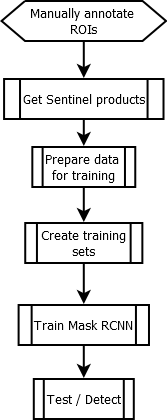
\includegraphics[width=.2\textwidth]{pics/overview.PNG}
  \caption{Gesamtablauf der Anwendung}
  \label{fig:overview}
\end{figure}
Zuerst müssen die Daten für das Training bzw. für die Erkennung manuell annotiert werden. Diese Metadaten werden dann genutzt, um automatisch Sentinelprodukte\footnote{Aufnahmenpakete der Sentinel-Plattformen werden als Produkte bezeichnet.} mittels einer API, die von der Copernicus zur Verfügung gestellt wird, herunterzuladen. Aus den Produkten werden die relevanten Bänder extrahiert und unter anderem die jeweiligen NDVI-Werte berechnet. Nachdem die Produkte für das Training vorbereitet wurden, werden die Daten in ein Trainings- und in ein Validierungsdatensatz aufgeteilt. Der folgende Trainingsprozess basiert auf diesen Datensätzen. Sobald das Training abgeschlossen ist, kann die Performanz des Modells getestet werden. 

\section{Annotation}\label{sec:annotation}

Zu Beginn werden die Regionen, die entweder für das Training benutzt oder überprüft werden, manuell erfasst. Vorrausgesetzte Informationen sind
\begin{itemize}
	\item Geografische Koordinaten,
	\item Zeitraum des Befalls und
	\item Bezeichnung der Infektion.
\end{itemize}
Als Format dieser Informationen dient \textit{GeoJSON}\footnote{GeoJSON ist eine Erweiterung des JSON-Format und beschreibt geografische Daten und Geometrien. GeoJSON wird durch den RFC7946-Standard definiert.}. GeoJSON enthält nicht nur geografische Daten, sondern ist auch um benutzerdefinierte Eigenschaften (\texttt{properties}) erweiterbar. Die Annotationen sind also GeoJSON-Features, die ein geografisches Polygon mit Metadaten enthalten.

\begin{lstlisting}[language=json,caption={Annotation},captionpos=b]
{
  "type": "Feature",
  "properties": {
    "disease": 1,
    "from": "2018-07-12T13:00:00Z-7DAYS",
    "to": "2018-07-12T13:00:00Z+7DAYS"
  },
  "geometry": {
    "type": "Polygon",
    "coordinates": [[[11.171988617177981,44.574291380353003],
       [11.1726616444942,44.574017992242283],
       [11.17338129910439,44.575068359984279],
       [11.17273129334275,44.575299863118993],
       [11.171988617177981,44.574291380353003]]]
  }
}
\end{lstlisting}
\noindent
\texttt{properties.disease} enthält die eindeutige, nummerische Repräsentation der Klasse bzw. Krankheit, die in dieser Region enthalten ist. Die Zuordnung der nummerischen Werte und des textuellen Bezeichners werden in einer separaten JSON als Schlüssel-Wert-Paare konfiguiert, wobei der Schlüssel nummerisch und der Wert textuell ist. Hier ist, darauf zu achten, dass der Schlüssel $\ge1$ ist, da $0$ der implizite Schlüssel der Mask R-CNN-Implementierung für den Hintergrund ist. Diese Eigenschaft ist nur für das Training von Relevanz.
\\\\
\texttt{properties.from} und \texttt{properties.to} sind jeweils Start- und Endzeitpunkt, in dem nach verfügbaren Sentinelprodukten gesucht werden soll. Das Format der jeweiligen Eigenschaften kann eine der folgenden Formen haben\footnote{Die Formate basieren auf der \texttt{sentinelsat}-Version 0.12.2.}:
\begin{itemize}
	\item \texttt{yyyyMMdd}
	\item \texttt{yyyy-MM-ddThh:mm:ss.SSSZ} (ISO-8601)
	\item \texttt{yyyy-MM-ddThh:mm:ssZ}
	\item \texttt{NOW}
	\item \texttt{NOW-<n>DAY(S)} (oder \texttt{HOUR(S)}, \texttt{MONTH(S)}, usw.)
	\item \texttt{NOW+<n>DAY(S)}
	\item \texttt{yyyy-MM-ddThh:mm:ssZ-<n>DAY(S)}
	\item \texttt{NOW/DAY} (oder \texttt{HOUR}, \texttt{MONTH} usw.) - Der Wert wird auf den jeweiligen Typ (z.B. auf den Tag) gerundet.
\end{itemize}
\noindent
Es ist angebracht einen Zeitraum von mehreren Tagen bzw. Wochen zu wählen, da die Sentinel-2-Satelliten keine täglichen Daten liefern und weil eine Infektion typischerweise über einen längeren Zeitraum vorherrscht. Die Zeitspanne ist von der Krankheit abhängig. Hier wurden eine Woche vor und nach dem Aufnahmezeitpunkt genutzt, um nach Produkten zu suchen.

\section{Suche nach Sentinelprodukte}


Der \textit{Copernicus Open Access Hub}\footnote{\url{https://scihub.copernicus.eu/}} ermöglicht freien und offenen Zugriff auf Sentinel-Produkte. Die Daten sind sowohl über eine grafische Oberfläche als auch über eine REST-API verfübar. Vorrausgesetzung für beide Optionen ist ein Account, der über die grafische Oberfläche erstellt werden kann.
\\\\
Die Nutzung der Schnittstelle erfolgt über die Python-Bibliothek \texttt{sentinelsat}\footnote{https://sentinelsat.readthedocs.io/en/stable}. Bei einer Anfrage müssen die GeoJSON-Dateien in WKT\footnote{WKT (Well-known text) ist eine Markup-Sprache zur Repräsentation von geometrischen Objekten auf Karten und räumlichen Referenzsystemen.} umgewandelt werden, was von der Bibliothek übernommen werden kann. Die WKT-Geometrie wird als \textit{footprint} (dt.: Fußabdruck) bezeichnet. Solang es nicht anders angegeben wird, gibt die Corpernicus-API Produkte zurück, die die RoI schneiden. Desweiteren wird der Plattformname statisch als `Sentinel-2' definiert, damit keine Produkte von den anderen Sentinelplattformen zurückgegeben werden. Der Suchzeitraum wird aus der jeweiligen GeoJSON-Datei übernommen. Sollten für die Suchanfragen keine Produkte existieren, wird die Anwendung beendet, da es keine Basis gibt, auf der das Netzwerk trainiert werden kann. Eventuell muss bei so einem Fall der Zeitraum erweitert und Prozess wiederholt werden. Bei vorhandenen Produkten lädt das Skript diese herunter. Die Produkte werden in einem komprimierten Format geliefert und enthalten neben zusätzlichen Informationen, Banddaten in separaten Dateien im JPEG2000-Format\footnote{JPEG 2000 genau wie GeoTIFF ist ein Bildformat in dem auch Metadaten abgelegt werden können. So sind Pixel geografischen Koordinaten zuordbar.}.
\\\\
Für jedes Produkt, das zur aktuellen Annotation gehört, wird ein neuer Eintrag zu einer \textit{FeatureCollection} hinzugefügt. Für die spätere Entwicklung sind die Annotationen so leichter zu finden und bearbeitbar. Außerdem bleiben dadurch die Originaldaten unberührt. Dieser Schritt wird für jede vorhandene Annotationsdatei wiederholt. Anschließend werden die Bilddateien für B4 und B8 aus dem Produkt extrahiert.

\begin{figure}[ht]
  \centering
  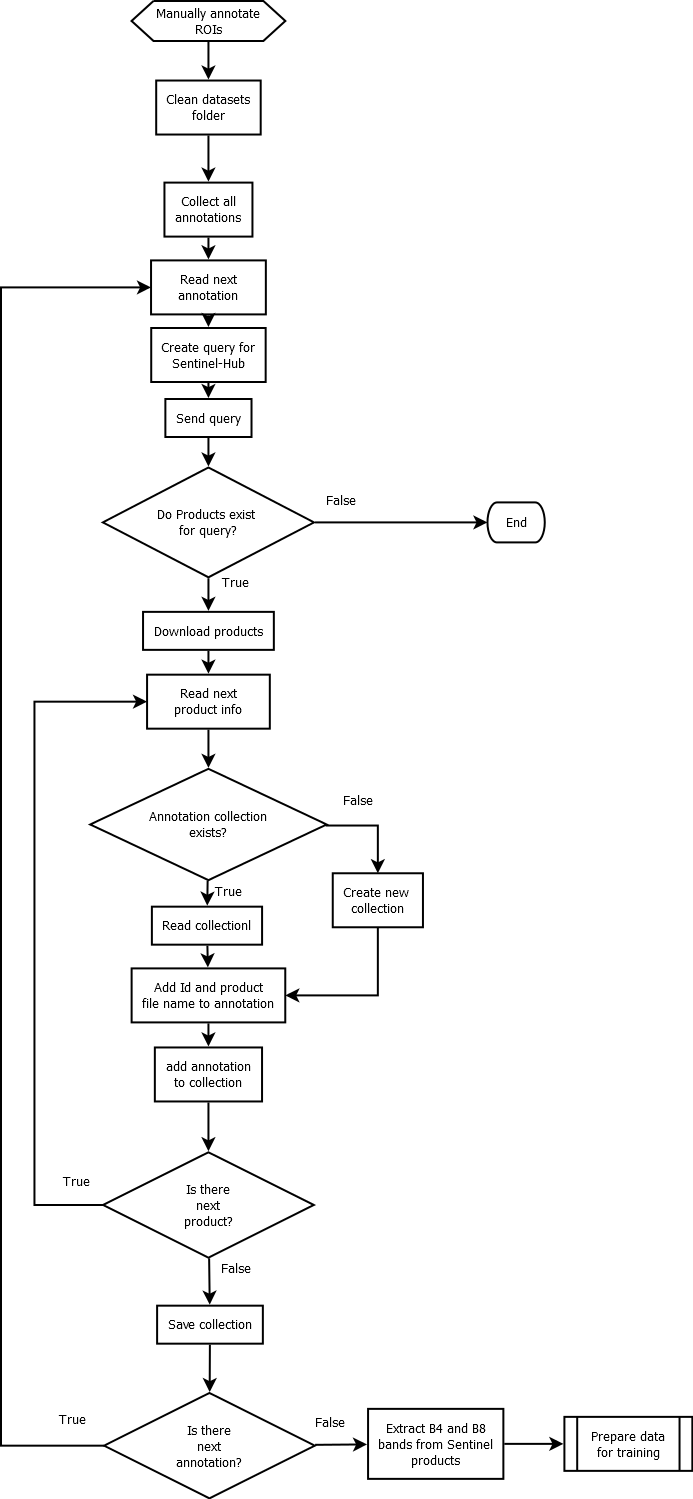
\includegraphics[height=\textheight-31pt]{pics/get-products.png}
  \caption{Ablaufdiagramm der Beschaffung der Sentinelprodukte}
  \label{fig:get-products}
\end{figure}

\section{Aufbereitung der Sentineldaten}

Originale Sentinel-2-Aufnahmen haben eine Größe von $10980*10980$ px und müssen deshalb deutlich verkleinert werden, um Speicherressourcen zu minimieren. Vor allem da nur kleine Ausschnitte von wenigen Pixeln benötigt werden. 
\\\\
Zu Beginn werden alle Elemente aus der vorher erstellten \textit{FeatureCollection} geladen und nacheinander bearbeitet. Jedes Produkt hat ein eigenes Koordinatenreferenzsystem (CRS, Coordinate Reference System) und unter Umständen unterscheiden sich die Systeme des Produktes und des Polygons\footnote{Nach RFC 7946 ist das geografische Referenzsystem \textit{World Geodetic
 System 1984} (WGS 84) das Standardsystem.\cite{ref:rfc7946}}. Diese müssen gleich sein, um miteinander agieren zu können. Das Produkt-CRS kann aus den extrahierten Bändern gelesen und dann dazu genutzt werden, um die Annotationskoordinaten in eben dieses zu projizieren.
 \\\\
 Nachdem abgesichert wurde, dass die RoI in dem Sentinelprodukt enthalten ist, wird aus den Bändern die RoI samt einem vorher definierten Rand ausgeschnitten. Der Rand ist später bei der Data Augmentation hilfreich. Gleichzeitig erstellt die Anwendung eine gleich große binäre Maske, wobei die Elemente der Maske mit den Pixeln der RoI korrespondieren. Die Elemente, die die RoI repräsentieren, enthalten einen wahren Wert.
 \\\\
\begin{figure}[ht]
  \centering
  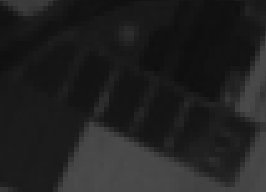
\includegraphics[height=3cm]{pics/b4.PNG}
  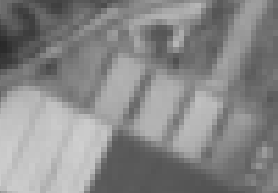
\includegraphics[height=3cm]{pics/b8.PNG}
  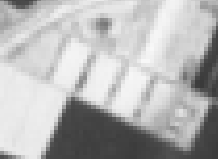
\includegraphics[height=3cm]{pics/ndvi.PNG}
  \caption[B4 - B8 - NDVI]{V.l.n.r. B4 (RED), B8 (NIR), NDVI}
  \label{fig:ndvi}
\end{figure}
\noindent
Nun wird der NDVI aus den B4- und B8-Ausschnitten, wie in Kapitel \ref{sec:ndvi} gezeigt, berechnet (s. Abb. \ref{fig:ndvi}). Das Ergebnis wird nun mittels Data Augmentation vervielfältigt. Dazu wird es vier mal um 90\degree gedreht. Danach wird jedes rotierte Bild horizontal und vertikal gespiegelt. Darauf werden zehn mal aus den rotierten und gespiegelten Daten zufällig Bilder in der Größe von $16*16$ px ausgeschnitten. Durch diese Operationen vergrößert sich die Grundgesamtheit um den Faktor 80. Jede Operation wird ebenfalls auf die entsprechende Maske angewandt.

\begin{figure}[ht]
  \centering
  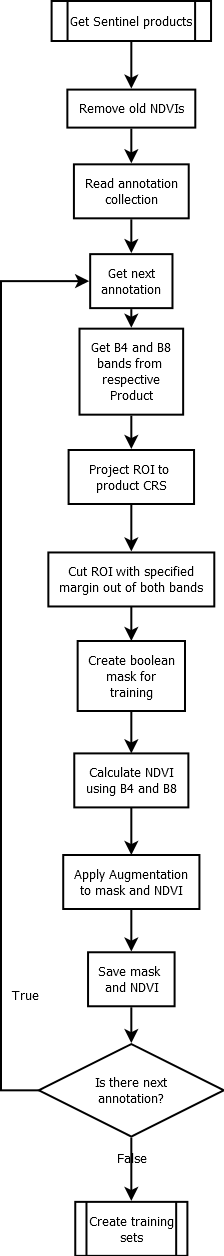
\includegraphics[height=0.95\textheight]{pics/create-ndvi.png}
  \caption{Ablaufdiagramm der Aufbereitung}
  \label{fig:create-ndvi}
\end{figure}

\section{Trainings- und Validierungsdatensatz}